\subsection{util}
\label{subsec:util}

\begin{figure}[H]
  \centering
  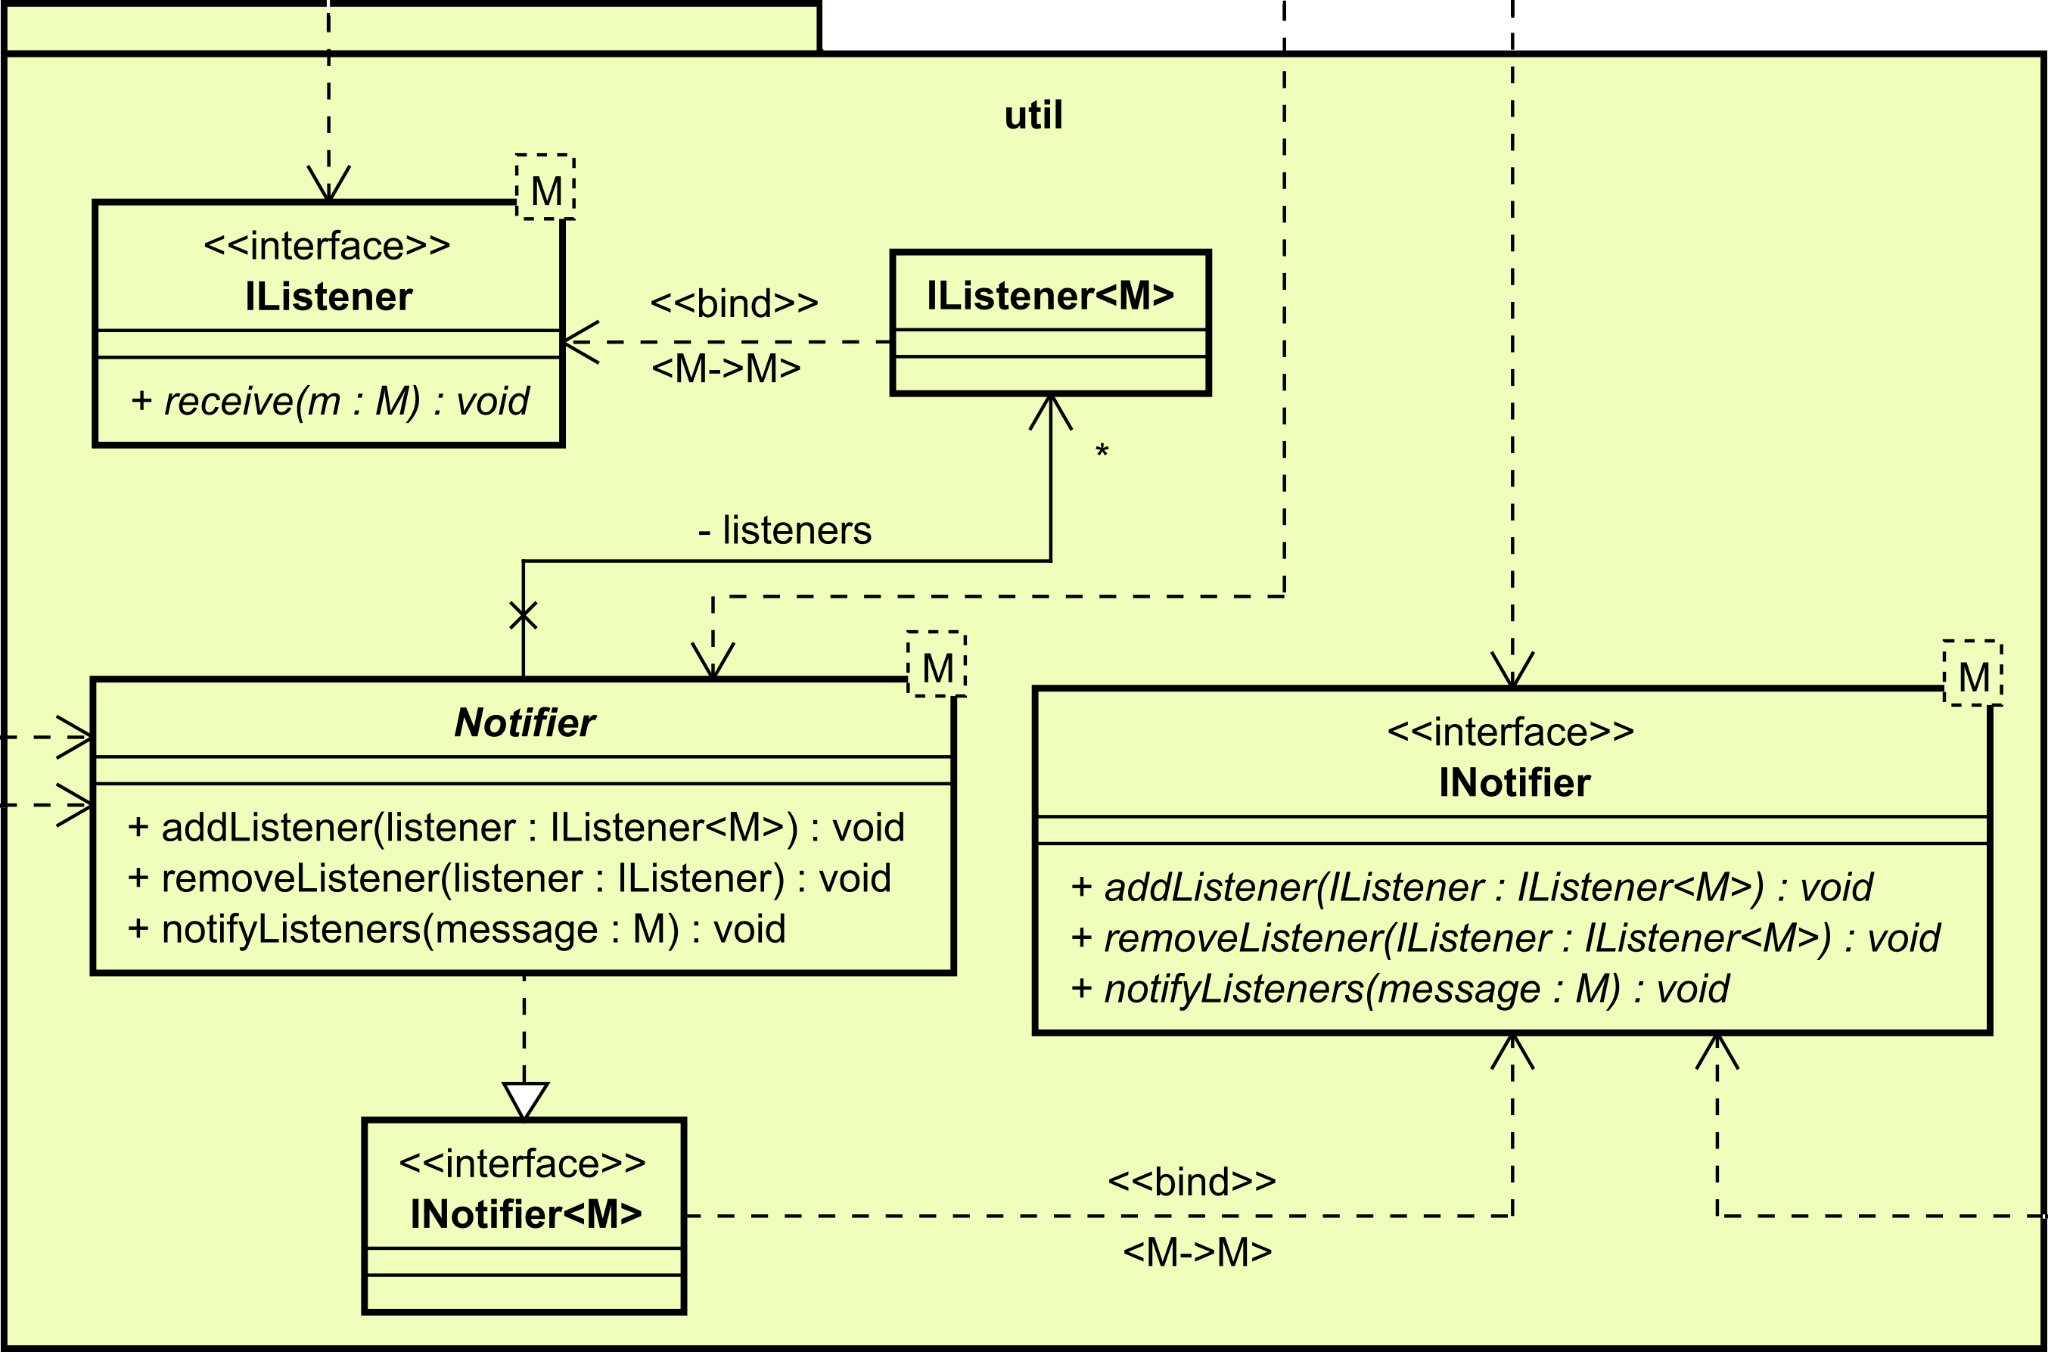
\includegraphics[width=\textwidth]{../diagramimages/util.png}
  \caption{util-Package}
\end{figure}

\medskip
Im util-Package befinden sich Klassen, die komplett von \gls{programname} abgekoppelt
sind. D.h. sie werden nur als Ressource, wie eine Liste, benutzt und nehmen kein
Bezug auf das Programm.\newline
Konkret befinden sich 3 Klassen im util-Package, die alle zusammen eine
Variation des \gls{observerpattern}s realisieren. Der \textit{Notifier} ist dazu da
ein beliebiges Objekt zu verschicken, deshalb der Generic. Er ist das Subjekt aus
dem \gls{observerpattern}.
\newline
\newline
Der \textit{INotifier} existiert für den Fall, dass ein
Objekt ein Notifier sein muss, aber nicht Notifier vererben kann, weil es
schon eine andere Klasse bererbt. Dieses Problem tritt beispielsweise im
\hyperref[subsec:view]{view}-Package auf, wo viele Klassen \gls{gui}-Aktionen als Commands
gekapselt an den Executor verschicken und gleichzeitig JavaFX Klassen bererben müssen.
Um dieses Problem zu lösen implementieren diese Klassen das INotifer-Interface
und haben ein Hilfsobjekt, das Notifier vererbt um somit die gewünschte Funktionalität zu
bieten.
\newline
\newline
Der \textit{Listener} ist der Beobachter aus dem \gls{observerpattern}. Hier ist nichts
besonders vaiiert worden, mit Ausnahme der receive-Methode, bei der wir einen Parameter eingeführt
haben damit der Listener das versendete Objekt des \gls{notifier}s auch empfangen kann.
Zu diesem Zweck existiert auch wieder ein Generic.
\newline
\newline
Dieses \gls{observerpattern} verwaltet das Verschicken und Empfangen von Commands in
\gls{programname}. In anderen Worten, jede Klasse, die Commands verschickt, ist ein
\gls{notifier}, und jede Klasse, die Commands empfängt, ist ein \gls{listener}. Dieses Design
hat große Vorteile, da die Sender und die Empfänger komplett voneinander abgekoppelt
sind. Der \hyperref[subsec:presenter]{Presenter} registriert die \gls{listener} bei Programmstart
bei den \gls{notifier}n, somit kennt der \gls{listener} nicht seinen \gls{listener}, und der
\gls{notifier} weiss nicht, was sich hinter einem \gls{listener} versteckt. Durch diese lose
Kopplung ist es einfach \gls{programname} um einen zusätzlichen Service zu erweitern,
da kein Service wirklich von einem anderen abhängt.
\newline
\newline
Ein Beispiel dieser losen Kopplung kann man zwischen dem
\hyperref[subsubsec:packetdataprocessor]{packetdataprocessor}-Package, dem
\hyperref[subsubsec:executor]{executor}-Package, und dem
\hyperref[subsubsec:replaylogging]{replaylogging}-Package finden. Hier erstellt
der Truffleprocessor neue Commands, die sowohl von dem Executor als auch von dem
ReplayLogSaveService empfangen werden sollen. Obwohl die 3 Packages sehr viel
mit einander zu tun haben, kenne sie sich gegenseitig nicht. Dieses Design
trägt zur Modularität von \gls{programname} bei.